\begin{frame}
\frametitle{Model-based dimensionality reduction}
Nonlinear dimensionality reduction techniques related to PCA:
\begin{itemize}
\item {\bf Principal geodesic analysis} combines PCA with image registration to maximise the amount of signal explained.\par
\begin{tiny}
Zhang, Miaomiao, and P. Thomas Fletcher. ``Bayesian Principal Geodesic Analysis in Diffeomorphic Image Registration.'' Medical Image Computing and Computer-Assisted Intervention--MICCAI 2014. Springer International Publishing, 2014. 121-128.\par
\end{tiny}
\item {\bf Non-negative matrix factorization} decomposes data into matrices that are non-negative.\par
\begin{tiny}
Lee, Daniel D., and H. Sebastian Seung. ``Learning the parts of objects by non-negative matrix factorization.'' Nature 401.6755 (1999): 788-791.\par
Sotiras, Aristeidis, Susan M. Resnick, and Christos Davatzikos. ``Finding imaging patterns of structural covariance via Non-Negative Matrix Factorization.'' NeuroImage 108 (2015): 1-16.\par
\end{tiny}
\item {\bf Generalized principal components} incorporates a link function into principal component analysis.\par
\begin{tiny}
Collins, Michael, Sanjoy Dasgupta, and Robert E. Schapire. ``A generalization of principal components analysis to the exponential family.'' Advances in neural information processing systems. 2001.\par
Mohamed, Shakir, Zoubin Ghahramani, and Katherine A. Heller. ``Bayesian exponential family PCA.'' Advances in Neural Information Processing Systems. 2009.\par
\end{tiny}
\end{itemize}
\end{frame}

\begin{frame}
\frametitle{Missing data}
\begin{columns}
\column{0.6\textwidth}
\begin{itemize}
\item Brain images of different individuals have different fields of view.
\item Currently, if test subject has smaller field of view than training data, the pattern recognition approch needs to be retrained.
\item Improved generative modelling could be used to better deal with missing data.
\end{itemize}
\column{0.4\textwidth}
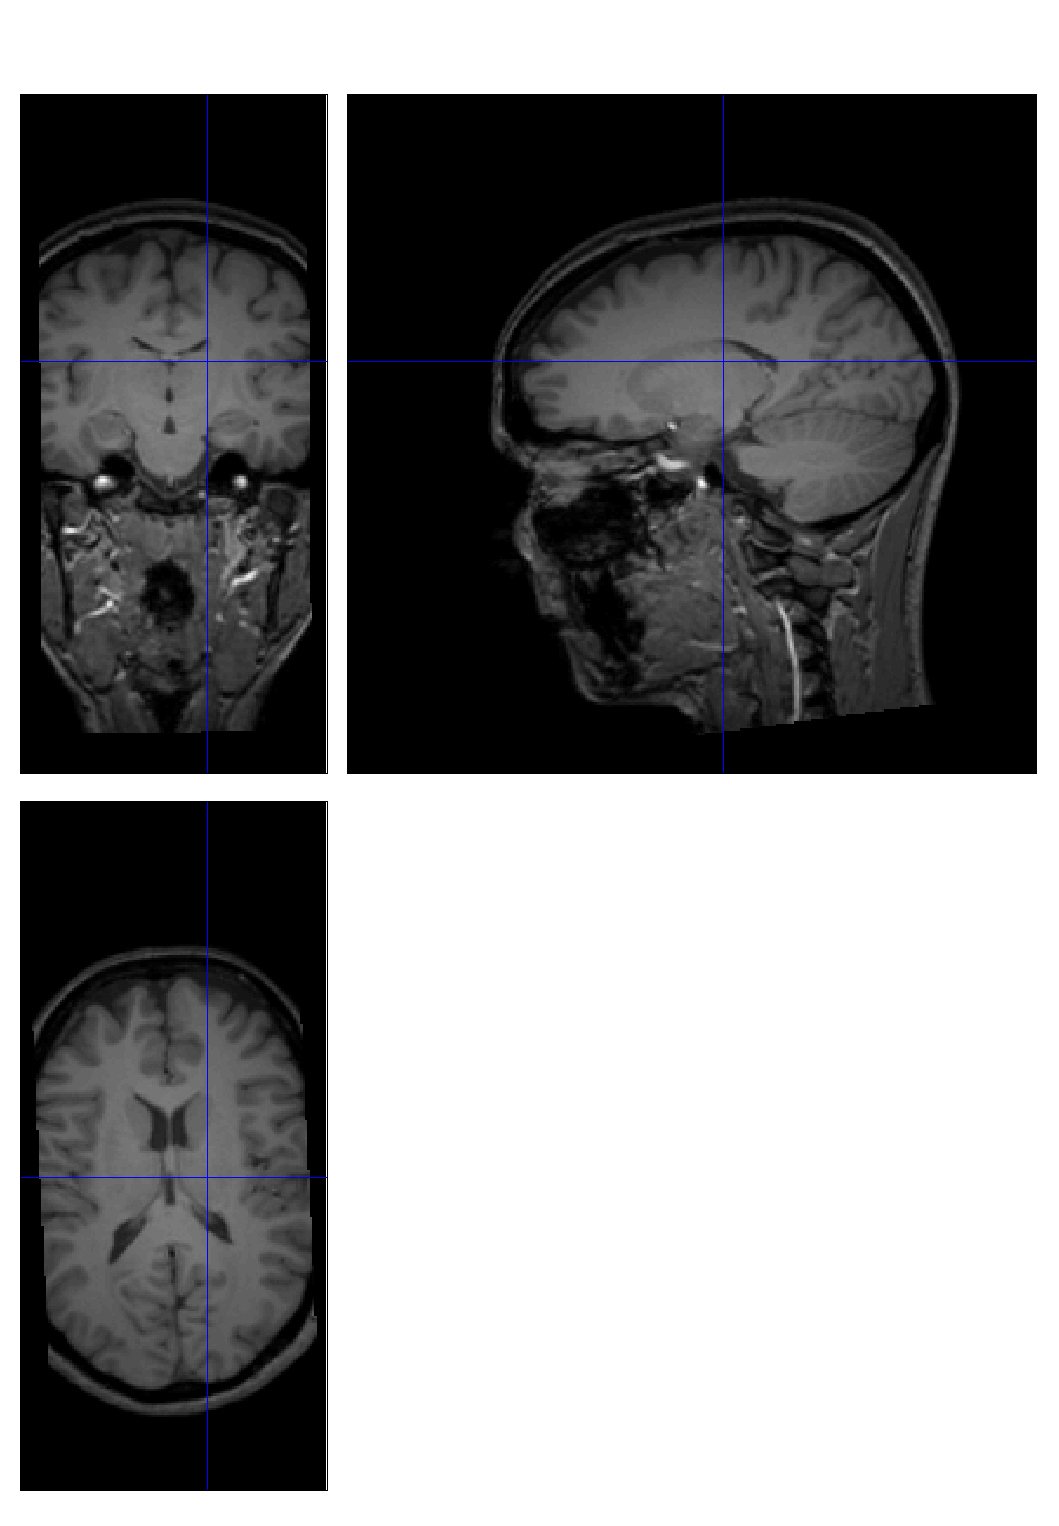
\includegraphics[width=\textwidth]{missing_slices}
\end{columns}
\end{frame}

\begin{frame}
\frametitle{Principled similarity measures}
How do we best compute similarity from models used to ``pre-process'' data?
\begin{itemize}
\item {\bf Fisher kernels} T. S. Jaakkola and D. Haussler. ``Exploiting generative models in discriminative classifiers.'' In Kearns et al. [26], pages 487--493.
\end{itemize}
\end{frame}

